\documentclass[12pt, a4 paper]{article}
% Set target color model to RGB
\usepackage[inner=2.0cm,outer=2.0cm,top=2.5cm,bottom=2.5cm]{geometry}
\usepackage{setspace}
\usepackage[rgb]{xcolor}
\usepackage{environ}
\usepackage{verbatim}
\usepackage{subcaption}
\usepackage{outlines}
\usepackage{enumitem}
\usepackage{amsgen,amsmath,amstext,amsbsy,amsopn,tikz,amssymb,tkz-linknodes}
\usepackage{fancyhdr}
\usepackage{pgfplots}
\usepackage{mathtools}
\usepackage[colorlinks=true, urlcolor=blue,  linkcolor=blue, citecolor=blue]{hyperref}
\usepackage[colorinlistoftodos]{todonotes}
\usepackage{rotating}

\linespread{1.6} % Double Line Spacing
\usetikzlibrary{arrows.meta,intersections,calc}

\hypersetup{%
pdfauthor={Vignesh Ravibaskar},%
pdfcreator={PDFLaTeX},%
pdfproducer={PDFLaTeX},%
}

% Our custom enumerate labelling, just making the outlines bold basically
\setlist[enumerate,1]{label=\textbf{\arabic*}}
\setlist[enumerate,2]{label=\textbf{({\alph*})}}
\setlist[enumerate,3]{label=\textbf{({\roman*})}}

\title{Maclaurin's Series}
\author{Derek, Vignesh}
\date{2020}

\newcommand{\comm}[1]{}
\NewEnviron{answer}{\vspace{3mm} \\ \color{blue} {\BODY} \color{black}}
%\NewEnviron{answer}{\color{blue} \comm{\BODY} \color{black}} % Use this method to hide all answers

\begin{document}

\maketitle

\textbf{MACLAURIN'S SERIES [TBC Marks]}
\begin{outline}[enumerate]
 \1 Sector \(AOB\) of a circle centred at \(O\) with radius 4 cm is such that \(\sphericalangle AOB = \frac{2\pi}{3}+\theta \) as shown in the diagram below: %Question 1
 \[
  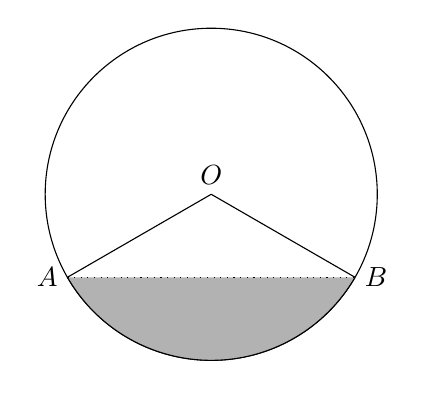
\begin{tikzpicture}
   \draw (0,0) node[above]{\(O\)} circle (60pt);
   \draw (-51.96152pt,-30pt) node[left]{\(A\)} -- (0,0);
   \draw (51.96152pt,-30pt) node[right]{\(B\)} -- (0,0);
   \filldraw[color=white!70!black,draw=black] (-51.96152pt,-30pt) arc (210:330:60pt);
   \draw[dotted](-51.96152pt,-30pt) -- (51.96152pt,-30pt);
  \end{tikzpicture}
 \]
 Given that \(\theta \) is sufficiently small for \(\theta^3\) and higher powers of \(\theta \) to be neglected, find the approximate area of the shaded region in terms of \(\theta \).\hfill[5]

 \1 It is given that \(y=\sqrt[3]{(1+x^2)(1+4x^2)}\). %Question 2

 \2 State the Maclaurin's expansion of \(y\) in ascending powers of \(x\) up to and including the \(x^4\) term.\hfill[4]

 \2 Hence, show that \(\frac{91487}{90000}\) is an accurate estimate for \(\sqrt[3]{1.0504}\)  up to 4 d.p..\hfill[2]

 \1 Given that \(y=2^{\sin^{-1}{x}}\), where \(\sin^{-1}{x}\) denotes the principal value, show that
 \begin{equation*}
  \dfrac{\mathrm{d}^2y}{\mathrm{d}x^2}=\dfrac{1}{y}{\left(\dfrac{\mathrm{d}y}{\mathrm{d}x}\right)}^2+\dfrac{1}{2x^2-2}\cdot \dfrac{\mathrm{d}y}{\mathrm{d}x}.
 \end{equation*}\hfill[4] \\
 Hence, obtain the first three terms in the Maclaurin's series for \(y\).\hfill[3] %Question 3

 \1 Find the first three non-zero terms in the expansion of \(f(x)=-\dfrac{x}{\sqrt{4-x^2}}\) % Question 4

 \1 Use the below function, \(f(x)\) for the following question. % Question 5
 \begin{equation*}
  f(x) = \begin{cases}
   \mathrm{e}^{1/x^2}, & \textrm{for }  x\neq0 \\
   0                   & \textrm{for } x=0
  \end{cases}
 \end{equation*}
 \2 Show that the \(f(x)\) is not equal to its Maclaurin series
 \2 Graph the function in \textbf{(a)}, labelling clearly the points at/around the origin.

 \1 Given that \(\tan{2x}=a_{0}+a_{1}x+a_{2}x^2+\dots \), by using the fact that \(\sin{2x}=\cos{2x}\cdot \tan{2x}\), obtain the expansion of \(\tan{2x}\) in ascending powers of \(x\), up to and including the term in \(x^3\).\hfill[4] %Question 6

 \1 It is given that \(\textrm{f}(x)=\dfrac{a-b}{(1-ax)(1-bx)}\), where \(a,b>0\). %Question 7

 \2 By expressing \(\textrm{f}(x)\) in terms of partial fractions and considering their Maclaurin expansions, show that:
 \begin{equation*}
  \sum_{r=0}^{\infty}(a^{r+1}+b^{r+1})x^{r}
 \end{equation*}\hfill[4]

 \2 Hence or otherwise, prove that, if \(x^3\) and higher powers of \(x\) may be neglected, then \(\dfrac{2}{(1-ax)(1-bx)} \approx 7+29x+133x^2\).
 \hfill[2]

 \1 Find the Maclaurin's Series for \(\mathrm{e}^{ix}\) up to and including the coefficient of \(x^7\) \hfill[3]
 \begin{answer}
  Using the standard series provided in MF26:
  \begin{align*}
   \mathrm{e}^{ix} = 1 + ix - \frac{1}{2!}x^2 - i\frac{1}{3!}x^3 + \frac{1}{4!}x^4 + i\frac{1}{5!}x^5 - \frac{1}{6!}x^6 - i\frac{1}{7!}x^7+ \dots
  \end{align*}
 \end{answer}
 Hence, prove that \(\mathrm{e}^{ix} = \cos x + i\sin x\) \hfill[3] % Question 8
 \begin{answer}
  We notice that
  \begin{align*}
   \mathrm{e}^{ix} & = 1 + ix - \frac{1}{2!}x^2 - i\frac{1}{3!}x^3 + \frac{1}{4!}x^4 + i\frac{1}{5!}x^5 - \frac{1}{6!}x^6 - i\frac{1}{7!}x^7+ \dots                             \\
                   & = \sum_{r=0}^{\infty} \frac{{(-1)}^r x^{2r}}{(2r)!} + i\sum_{r=0}^{\infty} \frac{{(-1)}^r x^{2r+1}}{(2r+1)!} = \cos x + i\sin x \quad\textrm{(Shown)}\quad
  \end{align*}
 \end{answer}
\end{outline}

\end{document}
